\documentclass[]{IEEEconf}

\usepackage{graphicx}
\usepackage{hyperref}
\usepackage[utf8]{inputenc}
\usepackage[caption=false,font=footnotesize]{subfig} % for subfigures


\title{EPC Ausarbeitung}

\author{Florian }

\date{2024-02-29}

\begin{document}

\maketitle

%%% FLORIAN
\section{Application in image processing}
Image processing is a widespread technology that can be used in industries such as medicine, manufacturing or monitoring. The simulation is implemented using Python. The qualitative evaluation of the algorithms is based on the error metrics Structural-Similarity-Index (SSI), Peak-Signal-to-Noise Ratio (PSNR) as well as Median Error Deviation (MED), Normalized Median Error Deviation (NMED) and Mean Relative Error Deviation (MRED). The following secrions give a partial impression of how the implementation of the specific image processing algorithms works. The structure of the image processing is based on an 8-bit RCA.

\subsection{image blurring}
Image blurring is a frequently used image processing technique. The field of application lies in pre-processing for other image processing algorithms, such as feature extraction or edge detection. Image blurring is used as a filter to suppress noise in an image. In this application, a 3x3 Gaussian blurring filter was used, which was applied to the image using convolution.
Figure .x shows the results for the image blurring algorithm in exact and approximated version.
Table .x shows the relative performance of different approximations in relation to the exact version. It can be highlithed that our own Version is...

\begin{figure}[!htb]
	\centering
	\subfloat[original]{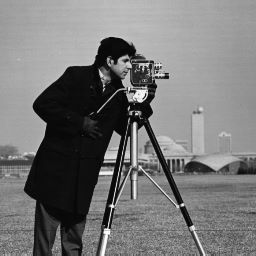
\includegraphics[width=0.3\linewidth]{cameraman.jpg}\label{fig:sub1}}\hfill
	\subfloat[correct blurred image]{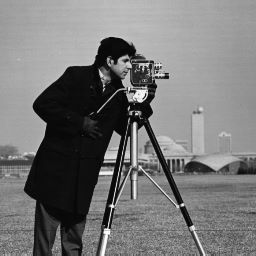
\includegraphics[width=0.3\linewidth]{cameraman.jpg}\label{fig:sub2}}\hfill
	\subfloat[approximated blurred image]{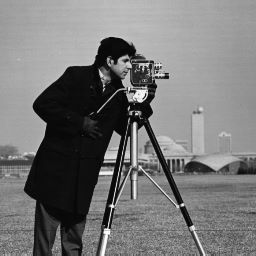
\includegraphics[width=0.3\linewidth]{cameraman.jpg}\label{fig:sub3}}
	\caption{image blurring results}
	\label{fig:whole}
\end{figure}% Image processing 

\subsection{edge detection}
edge detection is a fundamental image processing technique it is widely used to identify the boundaries of objects within an image. The edges represent significant color or intensity changes within the picture. The process of edge detection is done by applying a convolution with a here choosen laplacian kernel. In order to use the laplacian kernel, a twos complement algorithm was integrated so that addition and substraction can be performed one the same logic table. 


\begin{table}[h]
\caption{Error Metrics of the algorithm in a 8-bit RCA with different approximation degrees}
\begin{tabular}{|l|l|l|l|}
\hline
 Approximation Algorithm & MED & NMED & MRED  \\ \hline
Ax: 1/8 & 0 & 0 & 0 \\ \hline
Ax: 2/8 & 0 & 0 & 0 \\ \hline
Ax: 3/8 & 0 & 0 & 0 \\ \hline
\end{tabular}
\end{table}


\begin{table}[h]
\caption{Quality metrics of image processing applications}
\begin{tabular}{|l|l|l|l|l|}
\hline
Approximation Algorithm & image blurring & edge detection \\ \hline
Ax: 1/8 & 0 & 0 & 0 \\ \hline
Ax: 2/8 & 0 & 0 & 0 \\ \hline
Ax: 3/8 & 0 & 0 & 0 \\ \hline
\end{tabular}
\end{table}



\begin{figure}[!htb]
    \centering
    \subfloat[original]{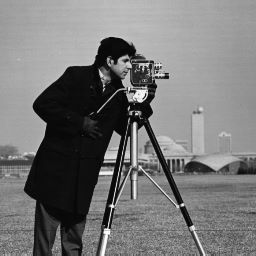
\includegraphics[width=0.3\linewidth]{cameraman.jpg}\label{fig:sub1}}\hfill
    \subfloat[correct edge detection]{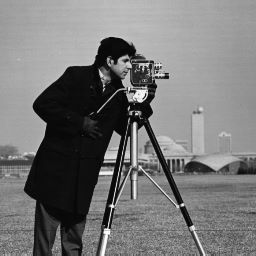
\includegraphics[width=0.3\linewidth]{cameraman.jpg}\label{fig:sub2}}\hfill
    \subfloat[approximated edge detection]{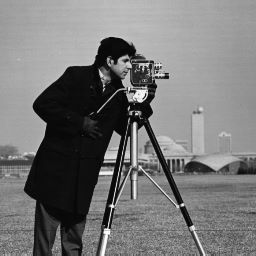
\includegraphics[width=0.3\linewidth]{cameraman.jpg}\label{fig:sub3}}
    \caption{Caption for the entire figure}
    \label{fig:whole}
\end{figure}% Image processing 

% Quality metrics 
% 	PSNR, SSI, MED, NMED, MRED, energy consumption

% Methods
% 	Image blurring
% 		Implementation, gausian blurr 
% 		Examples with quality metrics 
% 	Edge detection
% 		Implementation, twos complement
% 		Examples with qualitity metrics
% Application level comparison 

% Conclusion
		 


%%% Florian Ende


\end{document}